\documentclass[10pt,twoside,slovak,a4paper]{article}

\usepackage[slovak]{babel}
%\usepackage[T1]{fontenc}
\usepackage[IL2]{fontenc} 
\usepackage[utf8]{inputenc}
\usepackage{graphicx}
\usepackage{wrapfig}
\usepackage{url} % príkaz \url na formátovanie URL
\usepackage{hyperref} 

\usepackage{cite}
%\usepackage{times}

\pagestyle{headings}

\title{Problems of recommendation systems and their uncertain future\thanks{Semestrálny projekt v predmete Metódy inžinierskej práce, ak. rok 2024/25, vedenie: Yevheniia Kataieva }} 

\author{Dmytro Panychuk\\[2pt]
	{\small Slovenská technická univerzita v Bratislave}\\
	{\small Fakulta informatiky a informačných technológií}\\
	{\small \texttt{xpanychuk@stuba.sk}}
	}

\date{\small 28. oktober 2024} 



\begin{document}

\maketitle

\begin{abstract}
\centering

% \begin{table}
%     \begin{tabular}{l|r}
%         Item & Quantity \\\hline
%         First item  & First quantity  \\
%         Second item & Second quantity \\
%         Third item  & Third quantity  \\
%     \end{tabular}
%     \caption{Text for table}
%     \label{tab:widgets}
% \end{table}


Recommendation systems have become an incredibly important part of our lives. They are used in all online services, and the frequency of their use is only growing every year. 

These algorithms are used to personalise the experience by making suggestions tailored to our preferences and interests. The use of such systems is beneficial for both the platform and the end user. It recommends products that the user is more likely to buy, which saves them time and the platform will receive additional profit from new sales.  Without them, our modern online world would be impossible because it is a thing that allows the customer to find the product they need and the seller to increase sales through the target audience.

But these systems cannot be effective without users' personal information. This causes a lot of problems, both legal and moral. On the one hand, the user is not fully aware of how much of their personal information the platform receives, and on the other hand, databases are often hacked and your personal information can become public in a matter of seconds.

Also, the results of these systems are not always predictable. Sometimes, using recommendation systems can lead you into an “information bubble” from which you cannot get out without help. This can lead to terrible consequences that have already happened many times in human history. 

In this article, we will look at the problems of recommendation systems and the situations they have led to. We will also explore the methods of dealing with these problems that are used now and will be used in the future.
\newline
\newline
\newline
\end{abstract}


%  \begin{figure}[!h]
%     \centering
%     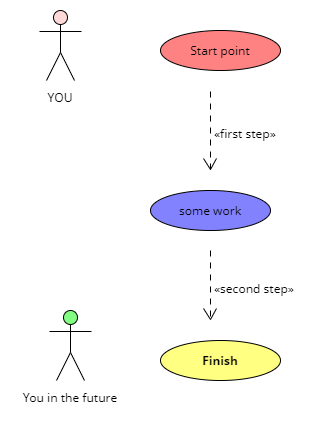
\includegraphics[width=0.7\linewidth]{Diagram.png}
%     \caption{Text for picture}
%     \label{fig:picture}
% \end{figure}



\section{Introduction}
In today's information society, where the amount of data and information is growing exponentially, users often face the problem of information overload. This phenomenon, known as ‘information overload’, makes it difficult to find the right products and services. In turn, sellers face difficulties in promoting their products in a competitive environment. Therefore, recommendation systems have become an integral part of modern business, as their main goal is to efficiently sort and select products according to individual user preferences.

Recommendation systems operate based on the analysis of user behavior, purchase history, product ratings and other factors. They use algorithms to predict whether a particular product is likely to appeal to a particular user based on previous preferences. In the digital world, such systems have become important tools for increasing customer satisfaction and driving sales for large e-commerce companies.

Well-implemented recommendation systems can significantly improve the user experience by making the shopping process more personalized and convenient. They help customers find the right products faster and expand their choices, which in turn helps to increase sales for businesses. Given these factors, the implementation of recommendation systems has become imperative for the successful operation of modern businesses.


While much has been written about the benefits of recommendation systems, the negative aspects of their use remain less well understood. These may include data privacy issues, algorithmic bias, and the risk of creating ‘information bubbles’ where users only receive content that confirms their existing views. This can lead to a limited diversity of information and products, which can negatively impact the user experience.

In this article, I plan to first describe in detail the general principles of recommendation systems~\ref{How They Work}, and then consider their varieties~\ref{Types of recommendation systems}, such as content-based recommendations, collaborative filtering, and hybrid approaches. Next, I will analyse the benefits that recommendation systems can provide to both users~\ref{Benefits for Users} and businesses~\ref{Benefits for Platforms}, highlighting their role in increasing customer satisfaction and sales performance.

Finally, I will focus on the challenges associated with recommendation systems~\ref{Ethical and Legal Issues} ~\ref{Risks of Data Breaches} ~\ref{Information Bubbles} and try to find possible solutions to these problems~\ref{Current and Future Solutions} ~\ref{Conclusion}. My suggestions will be based on research and innovations already being implemented by various companies and governments. This will include discussions on ethical standards, transparency of algorithms, and ways to ensure diversity in recommendations for users.




\section{How They Work} \label{How They Work}
 


\section{Types of recommendation systems} \label{Types of recommendation systems}

Základným problémom je teda\ldots{} Najprv sa pozrieme na nejaké vysvetlenie (časť~\ref{Types of recommendation systems:Collaborative filtering}), a potom na ešte nejaké (časť~\ref{Types of recommendation systems:Content-based filtering}).\footnote{Niekedy môžete potrebovať aj poznámku pod čiarou.}

Môže sa zdať, že problém vlastne nejestvuje\cite{Coplien:MPD}, ale bolo dokázané, že to tak nie je~\cite{Czarnecki:Staged, Czarnecki:Progress}. Napriek tomu, aj dnes na webe narazíme na všelijaké pochybné názory\cite{PLP-Framework}. Dôležité veci možno \emph{zdôrazniť kurzívou}.


\subsection{Collaborative filtering} \label{Types of recommendation systems:Collaborative filtering}

Niekedy treba uviesť zoznam:

\begin{itemize}
\item jedna vec
\item druhá vec
	\begin{itemize}
	\item x
	\item y
	\end{itemize}
\end{itemize}

Ten istý zoznam, len číslovaný:

\begin{enumerate}
\item jedna vec
\item druhá vec
	\begin{enumerate}
	\item x
	\item y
	\end{enumerate}
\end{enumerate}


\subsection{Content-based filtering} \label{Types of recommendation systems:Content-based filtering}

\paragraph{Veľmi dôležitá poznámka.}
Niekedy je potrebné nadpisom označiť odsek. Text pokračuje hneď za nadpisom.


\section{Benefits for Users} \label{Benefits for Users}


\section{Benefits for Platforms} \label{Benefits for Platforms}

\section{Ethical and Legal Issues} \label{Ethical and Legal Issues}

\section{Risks of Data Breaches} \label{Risks of Data Breaches}

\section{Information Bubbles} \label{Information Bubbles}

\section{Current and Future Solutions} \label{Current and Future Solutions}

\section{Conclusion} \label{Conclusion}


%\acknowledgement{Ak niekomu chcete poďakovať\ldots}

\bibliography{literatura}
\bibliographystyle{plain}
\end{document}
